Se busca poder realizar una implementación del \textit{algoritmo de Goertzel} en lenguaje C mediante el uso de \textit{S-Function} en MATLAB trabajando sobre el proyecto entregado como material de apoyo para la experiencia del laboratorio.


\begin{enumerate}
    \item Se crea la función \textit{computeGoertzel()} que recibe como argumentos el puntero al estado del filtro Goertzel y una muestra de entrada con el código que se muestra a continuación
    
    \begin{lstlisting}[language = C]
static double computeGoertzel(goertzelState_t *state,
                            double filterInput)

//Incrementa contador
	state->samplesCounter += 1;
//IIR
state->outputs[2] = state->outputs[1];
state->outputs[1] = state->outputs[0];
state->outputs[0] = filterInput + 
                    (state->A1)*state->outputs[1] 
                    - state->outputs[2];

//FIR
  if (GOERTZEL_N <= state->samplesCounter){
    state->binReal = state->cosW*state->outputs[1] 
                    - state->outputs[2];
    state->binImag = state->sinW*state->outputs[1];
    state->binMag = sqrt((state->binReal*state->binReal) 
                        +(state->binImag*state->binImag)  ); 

    resetGoertzel(state);
  }

	return state->binMag;
}

    \end{lstlisting}
    
    
    Otras funciones relevantes en el funcionamiento del algoritmo de Groetzel son aquellas que inicializan y reinician  los estados del filtro. La función \texttt{initGoertzel()} encargada de la inicialización se muestra a continuación, mientras que la función \texttt{resetGoertzel} solo reestablece en cero los valores del vector de salidas y el contador de muestras presentes en la estructura entregada para el laboratorio.
    
    \begin{lstlisting}[language = C]
static void initGoertzel(goertzelState_t *state, 
                        uint64_t kFrequency)
{
  state->samplesCounter 	= 0;
  state->cosW = cos(2*M_PI*kFrequency/GOERTZEL_N);
  state->sinW = sin(2*M_PI*kFrequency/GOERTZEL_N);
  state->A1  = 2*cos(2*M_PI*kFrequency/GOERTZEL_N);

  state->outputs[0] = 0.0;
  state->outputs[1] = 0.0;
  state->outputs[2] = 0.0;

  state->binReal =0.0;
  state->binImag=0.0;
  state->binMag = 0.0;

  return;    }
    \end{lstlisting}
    
    
    
El algoritmo de Goertzel entrega la magnitud de bines específicos en el espectro de una señal de N muestras, para evaluar el correcto funcionamiento de la implementación hecha se utiliza el archivo de audio \textit{dtmfSequence\_16\_16.wav}, para el cual se obtiene la DFT para los primeros 256 valores con el comando de MATLAB \textit{fft} y luego se grafica indicando el valor que resulta en los bines 8,9 y 10.  Por otro lado se simula el algoritmo con simulink y se analiza la primera muestra ( definida por los 256 primeros datos del archivo de audio) y se compara la magnitud presente en el gráfico de la DFT con la magnitud obtenida mediante simulación.

\begin{figure}[H]
    \centering
    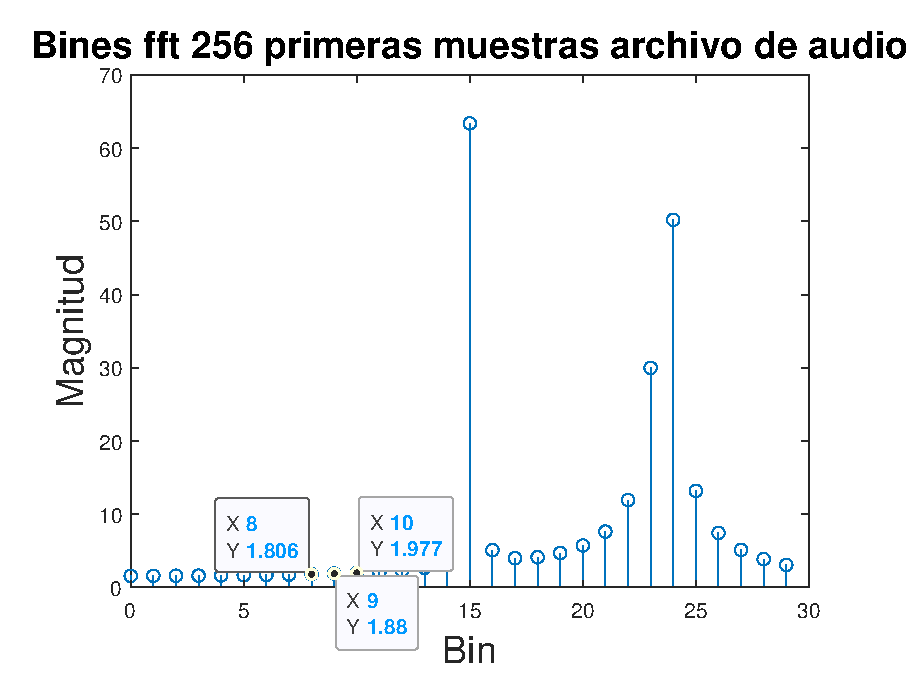
\includegraphics[width = .8 \linewidth]{Figuras/p7_1-fft_dtmf.eps}
    \caption{Gráfica de los bines obtenidos por la fft de las primeras 256 muestras del archivo de audio \textit{dtmfSequence\_16\_16.wav}.}
    \label{fft_256}
\end{figure}

\begin{figure}[H]
    \centering
    \includegraphics[scale = 0.4]{Figuras/7_1-mag-Goertzel.png}
    \caption{Magnitud de los bines 8, 9 y 10 asociados al archivo de audio  \textit{dtmfSequence\_16\_16.wav}, obtenidas mediante simulación.}
    \label{gotze_256}
\end{figure}


En la última figura las leyendas \textit{S-Function/1}, \textit{S-Function/2} y \textit{S-Function/3} corresponden a las magnitudes de los bines 8, 9 y 10 respectivamente. Comparando los valores que se muestran en el cuadro de datos a la derecha con los valores que indican los cuadros \textit{data tip} para los bines 8, 9 y 10 se puede ver que coinciden por lo que se concluye que la implementación del algoritmo de Goertzel funciona de manera correcta.


\item   Se instancia un total de 7 filtro Goertzel para lograr obtener los bins de frecuencia más cercanos a las frecuencias de los DTMF de la experiencia anterior, considerando el mismo archivo de usado anteriormente, el cual posee una frecuencia de muestreo de $16~ksps$ y nuevamente se analizan una cantidad N = 256 de muestras.

Para escoger correctamente los $k$ bins correspondiente a cada frecuencia DTMF se usa la expresión 

$$ k-Bin =  \frac{f_{DTMF} \cdot N}{Fs}$$ 

Redondeando de ser necesario el resultado, pues los $k- bines$ han de ser números enteros. De esta forma se obtiene la siguiente tabla



 \begin{table}[H]
        \centering
        \begin{tabular}{|c|c|}
        \hline
         frecuencia DTMF   & k-Bin  \\
         \hline
697  Hz & 11 \\
\hline
770  Hz & 12 \\
\hline
 852  Hz & 14\\
\hline

941  Hz & 15\\
\hline


1209  Hz & 19\\
\hline
 
941  Hz & 15\\
\hline
 
1336 Hz & 21\\
\hline

1336 Hz & 21\\
\hline

        \end{tabular}
        \caption{Cuadro resumen para el error cuadrático medio entre el resultado de la función \texttt{DFTsum} y el resultado entregado por el comando \texttt{fft} de MATLAB para cada señal de prueba.}
        \label{MSE}
    \end{table}
    
    
Se modifica la sección de código correspondiente quedando de la siguiente forma 

\begin{lstlisting}
 #define GOERTZEL1_K_BIN	    (11)
 #define GOERTZEL2_K_BIN	    (12)
 #define GOERTZEL3_K_BIN	    (14)
 #define GOERTZEL4_K_BIN	    (15)
 #define GOERTZEL5_K_BIN	    (19)
 #define GOERTZEL6_K_BIN	    (21)
 #define GOERTZEL7_K_BIN	    (24)
\end{lstlisting}


Usando los comandos \textit{subplot} y \textit{bar} se grafican los resultados para las 7 salidas de los filtros Goertzel, y tal como se esperaba, se cumple que en todo momento existen solo dos de las 7 componentes (bines) con magnitudes altas , correspondientes a las frfecuencias DTMF. Esta gráfica se muestra en la figrua \ref{dtmf}

\begin{figure}[H]
    \centering
    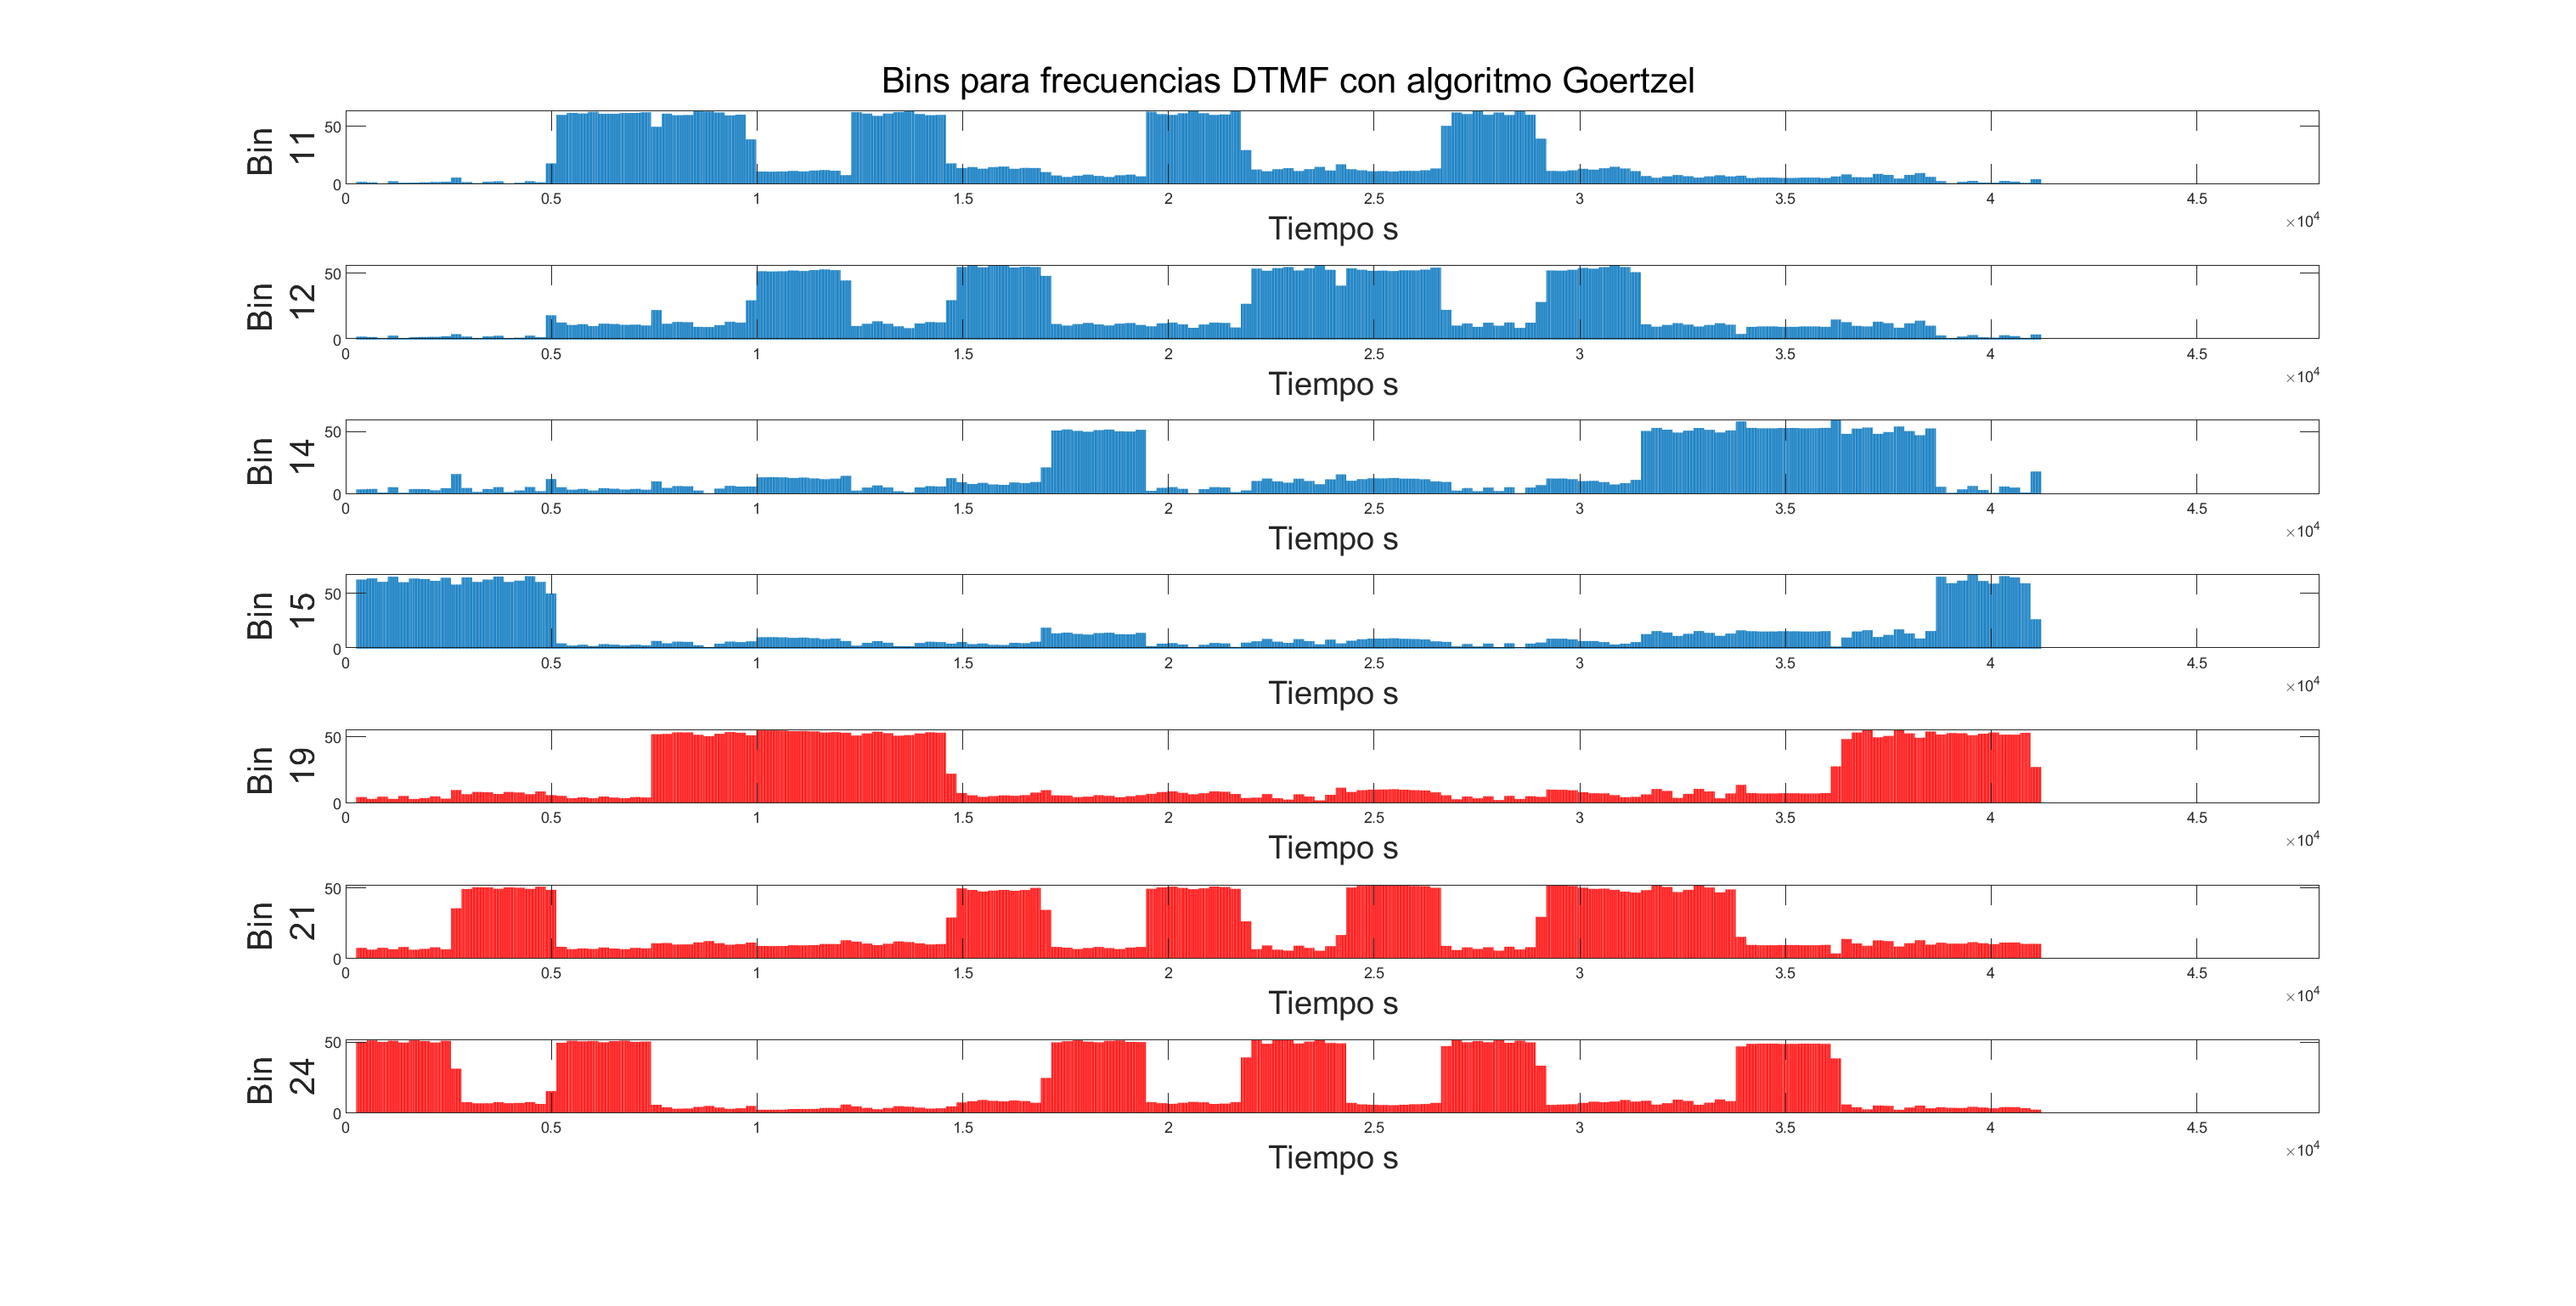
\includegraphics[scale = 0.35]{Figuras/p7_2.eps}
    \caption{Bins asociados a las frecuencias DTMF graficados en el tiempo usando el algoritmo de Goertzel}
    \label{dtmf}
\end{figure}

\end{enumerate}

  
  
  
  

  


